\section{印度佛教史}

\subsection{种性制度}
\begin{itemize}
  \item 婆羅門:祭司
  \item 剎帝利:武士
  \item 吠舍: 农工商业
  \item 首陀羅: 奴隶
\end{itemize}

\subsection{六派哲學}
產生於史詩時期之末,與佛教初期階段相近的婆羅門教哲學\footnote{木村泰賢$\cdot$《原始佛教思想論》}。
\begin{itemize}
  \item 尼夜耶派(The Nyāya School)。
  \item 僧佉耶派(The Sāṃkhya School)即數論派。
  \item 毘舍迦派(The Vaiśeṣika School)即勝論派。
  \item 瑜伽派(The Yoga School)。
  \item 弭曼差派(The Mīmāṃsā School)。
  \item 吠檀多派(The Vedānta School)。
\end{itemize}

\subsection{奧義書}
\begin{itemize}
  \item 業說,在《古奧義書》本為不公開的密教,到佛世則成為各教派所公認的思想
  \item 輪迴說,在梵書時代已萌芽,完成而為一般所承認,則自奧義書時代始
  \item 解脫說,乃為《奧義書》的最終目的
\end{itemize}

\subsection{六師外道}
記載常見於声闻經律\footnote{《長阿含經》第二十七經《沙門果經》}
\begin{itemize}
  \item 不蘭迦葉(Pūraṇa-Kāssapa):為倫理的懷疑者,否定善惡之業有其相應之根,故倡無作用論。
  \item 末伽梨瞿舍利(Makkhali Gosāla):此為邪命外道之祖,倡無因而有論。乃是耆那教的一派,在佛世極有勢力,除了耆那教,他是其餘五師中最盛大者。
  \item 阿耆多翅舍欽婆羅(Ajita Keśakambala):否定靈魂之說,倡唯物論,以快樂為人生之目的,排斥一切嚴肅的倫理觀念,此亦即是順世外道。
  \item 婆浮陀伽旃那(Pakudha Kaccāyana):主張心物永不消滅,倡世間常存論。
  \item 散若夷毘羅梨沸(Sañjaya Belaṭṭhiputta):為詭辯派或捕鰻論者,舍利弗(Śāriputra)及目犍連(Mahāmaudgalyāyana),即是此派出身而皈信佛教的。
  \item 尼乾陀若提子(Nigaṇṭha-Nātaputta):這就是耆那教之始祖摩訶毘盧(Mahā-vira),他出世稍早於釋尊,也是王子出身。此派以命(Jīva)及非命之(Ājīva)之二元論而說明一切,故也是否定有上帝造物觀念的無神論者。其實踐方面,則以極端的苦行及嚴守不殺生為特色。
\end{itemize}

\subsection{六十二見}
兩說及十類\footnote{《長阿含經》卷一四第二十一經《梵動經》}
\begin{itemize}
  \item 說過去世,或稱本劫本見者,五類十八見:
    \begin{itemize}
      \item 世間常住論,即是常見論,四種。
      \item 世間半常半無常論,四種。
      \item 世間有邊無邊論,四種。
      \item 異問異答論,即是詭辯派、捕鰻論、不死矯亂論,四種。
      \item 無因而有論,即是無因論,二種。
    \end{itemize}
  \item 說未來世,或稱末劫末見者,五類四十四見:
    \begin{itemize}
      \item 世間有想論,十六種。
      \item 世間無想論,八種。
      \item 世間非有想非無想論,八種。
      \item 眾生斷滅無餘論,即是斷見論,七種。
      \item 現法涅槃論,即無論在何種狀態,處於現世的即為最高的境界,五種。
    \end{itemize}
\end{itemize}

\subsection{家谱}
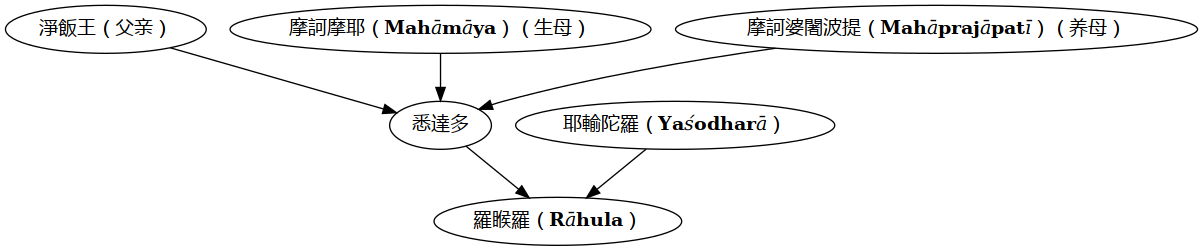
\includegraphics[width=\textwidth]{释家/images/释尊家谱.png}

\subsection{修道}
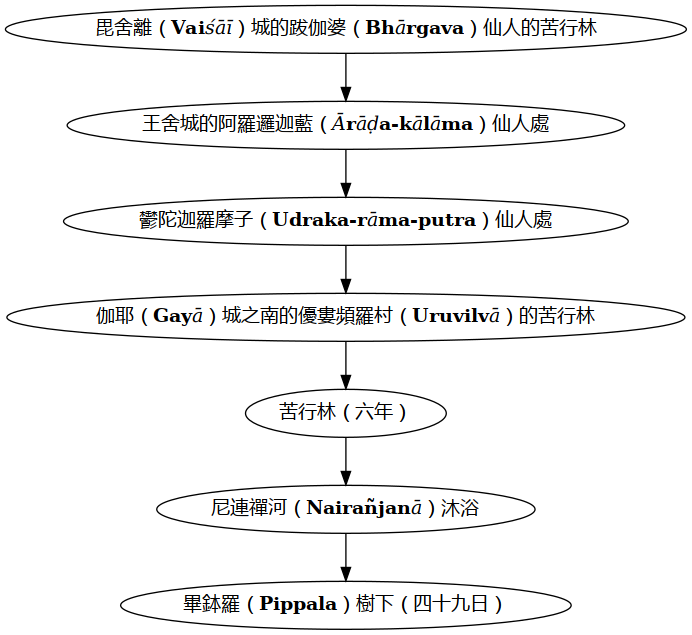
\includegraphics[width=\textwidth]{释家/images/释尊修行地图.png}

\subsection{四七日}
\begin{enumerate}
  \item 在菩提(Bodhivṛkṣa)樹下。就是那棵畢鉢羅樹之下,因佛在此樹下成道,而被稱為菩提樹
  \item 在阿踰波羅(Ajapāla)樹下。此期有魔王波旬(Māra-pāpīmān)來請佛入滅而未果。
  \item 在目真鄰陀(Mucilinda)樹下,遇暴風雨,目真鄰陀龍見之而即以己身護佛。此龍即受皈依,乃為傍生中的第一弟子。
  \item 在羅闍耶恆那(Rājāvatana)樹下。有二商主,一名提謂,一名婆梨迦,道經佛處,以麨蜜供佛,並皈依佛、法而去。此二人乃為最早的優婆塞(Upāsaka 親近而奉事三寶的淨信男)
\end{enumerate}

\subsection{轉法輪}
\begin{enumerate}
  \item 婆羅奈斯(Vārāṇiasī)城的鹿野苑度五比丘,接著又度了耶舍(Yaśa)及其親友數十人
    \footnote{ 阿若憍陳如(Ājñāta-Kauṇḍinỵa)、跋提(Bhadrika)、婆波(Vāṣpa)、摩訶男(Mahānāma)阿說示(Aśvajit)}
    \footnote{自此即有了教主、教法、教團的(佛、法、僧)三寶具足}
    \footnote{滿慈子、大迦旃延、婆毘耶等,亦捨外道法而進入佛法。}
    。
  \item 在鹿野苑度過第一個雨季的安居生活,釋尊便囑咐弟子們各各遊化人間,弘揚佛陀的教義
    \footnote{乃至要弟子們不應兩個人同走一條路};
    佛陀自己也單獨去到優婁頻羅聚落
    \footnote{化度了事火外道優婁頻羅迦葉(Uruvilvā-kāśyapa)和他的兩個弟弟那提迦葉(Nadī-kāśyapa)、伽耶迦葉(Gayā-kāśyapa),以及他們三人的弟子共一千人。}
    。
  \item 釋尊為了履行成道之後去度頻婆沙羅王的諾言,便率領迦葉三兄弟及其弟子們到了王舍城,國王
    \footnote{見到聞名於當時的迦葉三兄弟,均已成了佛的弟子,信心益加懇切,聞法之下,即得法眼淨(見道)。}
    親率臣民迎於郊外;迦蘭陀(Kalanda)長者將他在王舍城外的竹園施佛,王即為佛陀在此園中建造精舍
    \footnote{這是第一所大規模的佛教道場}
    。
  \item 佛陀成道第四年,六師外道之一的詭辯派的名匠舍利弗於言下
    \footnote{「諸法因緣生,諸法因緣滅」,「諸行無常,是生滅法,生滅滅已,寂滅為樂」}
    得法眼淨,和同門知友大目犍連各率弟子共二百五十人,詣佛出家,證阿羅漢果;
    又有摩訶迦葉(Mahā-kāśyapa)\footnote{「若不值佛,亦當獨覺。」}迴心進入釋尊的法海
    \footnote{佛經中常見的「千二百五十人俱,皆是大阿羅漢」的教團,到此便已形成。}
    。
  \item 佛陀成道第五年,即受到憍薩羅國(Kośala)首都舍衛城(Śrāvastī)的禮請,那就是須達(Sudatta 又作須達多)長者以重價購了一座祇樹給孤獨園奉施佛陀,作為弘法的中心。
  \item 同年,釋尊也應父王之召,回到祖國迦毘羅衛省親,父王預建精舍於尼拘律園,以接待釋尊。
    釋尊為父王說法,淨飯王即在聽法之際得法眼淨,宮人也多受了戒法,並度了異母弟(摩訶婆闍波提所生的)難陀,以及佛陀的親子羅睺羅出家。
    這次回國一共住了七天,便辭別父王返至王舍城,但卻在釋尊的座下,因此而增加了許多由釋迦王族來出家的弟子們
    \footnote{其中著名的,就有阿那律(Aniruddha)、阿難(Ānanda)、金毘羅(Kumbhīra)、提婆達多(Devadatta)等的追踪而至;為王子們理髮的賤民優波離(Upāli),亦於此時趕來出家,並且得到佛陀的特別優遇,讓他出家在諸王子之先,一則為表佛法的平等,一則為抑制諸王子驕傲的習氣。}
    \footnote{後世傳稱的佛陀的十大弟子,除了須菩提(Subhūti)似乎出家較遲而外,到此為止,其他的九位,均已出現了。}
    。
  \item 自釋尊成道第六年後,即沒有詳細的年月及活動的地點可考\footnote{《僧伽羅剎所集經》列記佛陀歷年雨安居的所在}。
  \item 經過四十五年的化度,召集全體比丘們在毘舍離的竹林精舍會齊,做最後一次重要的教誨;最後到了拘尸那羅城外的娑羅(Śāla)樹林入滅
    \footnote{一位叫作須跋陀羅(Subhadra)的外道成為佛陀最後得度的弟子。}
    \footnote{《長阿含經》卷四第二經《遊行經》:「是故比丘,無為放逸,我以不放逸故,自致正覺。無量眾善,亦由不放逸得。一切萬物,無常存者。此是如來末後所說。」}
    \footnote{《佛遺教經》:汝等比丘,常當一心,勤求出道,一切世間動不動法,皆是敗壞不安之相……是我最後之所教誨。」}
    。
\end{enumerate}


\subsection{原始佛教}
\begin{quote}
  是指佛陀在世時的言行,以及經過佛陀親自印可了的弟子們的言行。這唯有從《阿含經》及律部中去找,而《阿含經》比律部更可信賴。
\end{quote}
\begin{quote}
  開示的內容不外四聖諦、十二因緣、八正道等。
\end{quote}
\begin{quote}
  先以人天法,使你法天法人,使你成為一個可敬的人,當你善根增長皈依三寶,受持五戒之後,再用解脫法門開示你。人天善法是一般人共同信守的,解脫法門則是佛陀獨自證悟經驗的。
\end{quote}
\begin{quote}
  佛弟子們應當重視佛陀應化的重心,是著重於人生的修為而至無明的解脫,不必以為佛陀已將一切的問題給我們做了解答。佛陀的任務在此而不在彼,不要捨本逐末,否則自己鑽進了死角,還要埋怨,那是咎由自取。
\end{quote}
\begin{quote}
  佛陀既以人生的無明之解脫為著眼,人生的主宰則在於「心」,心不能自主,因為心的特性是念念相續地活動變異,故為無常,無常即無主體可覓,故為無我。
\end{quote}

\subsection{经典结集}
\subsubsection{第一次}
  迦葉尊者\footnote{錫蘭《大史》第三章}自佛涅槃地趕至王舍城,由於阿闍世王的外護,即在毘婆羅(Vebhāra)山側的七葉窟(Sapta-parṇa-guhā)前,建築精舍,集合五百位大比丘,作為佛滅後第一次的雨安居處。在此安居期間,自第二個月開始一連七個月(北傳謂三個月),從事結集的工作。首由優波離誦出律藏,次由阿難誦出法藏。此即稱為「五百集法毘尼」,或稱「王舍城結集」,又名「第一結集」
  \footnote{僅是迦葉一派的人,是少數人的結集,是代表上座比丘之中苦行派的一個大會。}
  ;當王舍城的結集終了,在南傳《善見律》、北傳《四分律》、《五分律》,都說有一位富蘭那長老\footnote{釋尊第七位比丘,是耶舍的四友之一, 而不是說法第一的富樓那。},率領了五百比丘從南方來到王舍城,亦說是南山(Dakkhiṇa-giri)來,重新與大迦葉論法及律。
  第一結集的戒律內容,便是代表上座精神的標記,並為上座們鞏固了領導的地位。
\subsubsection{第二次}
薩婆伽羅、離婆多、三菩提、耶舍、修摩那、沙羅、富闍蘇彌羅、婆薩摩伽羅摩,加上一位受戒僅五歲而堪任教化並精識法律的敷坐具之人阿耆多(或阿夷頭),共九人。
九人的審查辯論,實際是代表了七百人的大會,故此稱為七百結集。
\paragraph{十事非法的問題}
此一大會,起因雖為乞錢,討論內容則共有十項,稱為跋耆比丘的十事非法,那便是:
\begin{itemize}
  \item 角鹽淨:即是聽貯食鹽於角器之中。
  \item 二指淨:即是當計日影的日晷,未過日中之後(橫列)二指的日影時,如未吃飽,仍可更食。
  \item 他聚落淨:即在一食之後,仍可到另一聚落復食。
  \item 住處淨:即是同一教區(界內)的比丘,可不必同在一處布薩。
  \item 隨意淨:即於眾議處決之時,雖不全部出席,但仍有效,只要求得他們於事後承諾即可。
  \item 所習淨:隨順先例。
  \item 生和合(不攢搖)淨:即是得飲未經攪拌去脂的牛乳。
  \item 飲闍樓㘈淨:闍樓㘈是未發酵或半發酵的椰子汁,得取而飲之。
  \item 無緣坐具淨:即是縫製坐具,可不用貼邊,並隨意大小。
  \item 金銀淨:即是聽受金銀。
\end{itemize}
毘舍離的跋耆比丘,以此十事可行,為合法(淨)\footnote{「吾滅度後,應集眾僧,捨微細戒。」};
上座耶舍,則以此為不合律制,為非法\footnote{「隨佛所說,當奉行之,佛不說者,此莫說也。」}。
第二次結集的目的,即在審查此十事的律制根據。其結果,據各律典的記載,上座代表們一致通過,認為十事非法。

\subsubsection{第三次}
上座系所出的三說:
\begin{itemize}
  \item 犢子系的傳說:佛滅百三十七年,波吒釐子城有魔,名眾賢,作羅漢形,與僧共諍十六年,遂有犢子比丘,集和合僧而息其諍,那時的護法者,為難陀王。故名第三結集。
  \item 分別說系的傳說:佛滅二百三十年頃,華氏城(Pāṭaliputta)有賊住比丘起諍,阿育王迎目犍連子帝須(Moggaliputta-Tissa),集千比丘而息諍,是為第三結集。
  \item 一切有系的傳說,佛滅四百年,迦膩色迦王因信說一切有部,集五百大德於迦濕彌羅,集三藏而裁正眾多的異說。
\end{itemize}

\subsubsection{第四次}
根據傳說,正因有部思想的分歧,當佛滅四百年頃,迦膩色迦王為求其一致,遂請脇比丘及世友為上首,集合了五百羅漢,在迦濕彌羅進行了第四次的三藏結集。這次的成果,便是集體撰作了一部二百卷的《大毘婆沙論》。此論雖以統一的目的為出發,卻是站在那僕底(北印之東方)《發智論》的立場,對妙音的見解尚有所取捨,對犍陀羅(北印之西方)譬喻師的見解,則完全加以破斥。

\subsubsection{六部律藏}
\begin{itemize}
  \item 南傳上座部\footnote{上座部應先於大眾部,可是南方的上座部,實是上座部中偏於大眾部的分別說系之一支,故仍較《摩訶僧祇律》為後出,其他四部也屬上座部的分部所出,上座根本部的律藏,今已無從求得了。}的Vinayapiṭaka,巴利文。
  \item 大眾部的《摩訶僧祇律》四十卷,東晉佛陀跋陀羅共法顯譯。
  \item 化地部的《五分律》三十卷,劉宋佛陀什共智勝譯。
  \item 法藏部的《四分律》六十卷,姚秦佛陀耶舍共竺佛念譯。
  \item 摩偷羅有部的《十誦律》六十一卷,姚秦鳩摩羅什譯。
  \item 迦濕彌羅有部的《根本說一切有部毘奈耶》五十卷,唐義淨譯。
\end{itemize}

\subsubsection{法}
法的遞演,經過三期而後大定:
\begin{enumerate}
  \item 集佛陀的言行為九部經(九分教)
  \item 演九部經為四《阿含經》
  \item 依四《阿含經》而立雜藏\footnote{由雜藏而出大乘藏、禁咒藏,那是大乘的範圍了}。
\end{enumerate}
\paragraph{九部經}
\begin{itemize}
  \item 修多羅(Sūtra):即是散文的說法,通稱為長行。
  \item 祇夜(Geya):以韻文重將所說散文的內容頌出,通常譯為應頌或重頌。
  \item 伽陀(Gāthā):說法時全以韻文宣出,譯作孤頌或諷誦。
  \item 尼陀那(Nidāna):記述佛及弟子的事蹟、始終、本末,因以事緣常為說法之助緣,故譯為因緣。
  \item 阿鉢陀那(Avadāna):以譬喻說法,或凡因事而興感,皆名譬喻。
  \item 闍多伽(Jātaka):佛陀自說過去世的因緣,兼及重要弟子們的宿行,故稱為本生。
  \item 伊帝目多伽(Itivṛttaka):敍述古佛的化跡,故稱本事。
  \item 阿浮達摩(Adbhuta-dharma):明佛及弟子種種不思議的神跡奇行者,故稱未曾有,新譯為阿毘達磨。
  \item 優波提舍(Upadeśa):對於甚深而簡要的法義,用問答方式來解說,故稱為論義,後世的論藏,即脫胎於此。
\end{itemize}
在這九部經中,以前三部為最古而最近於原形佛典,故與今之《雜\footnote{雜為相應之意,乃為原始結集的舊制。}阿含經》相當;
至於第四部因緣至第八部之未曾有,此五部為釋尊景行之類集,性質與前三部大不相同\footnote{實則九部經的後六部,即由前三部中分出,初次結集時,是否已有九部之名,乃為近世學者置疑。}。
\paragraph{十二部经}
上九部之外,加上優陀那(Udāna)(即鄔陀南)即無問自說、毘佛略(Vaipulya)即方廣、和伽羅(Vyākaraṇa)即授記。

\subsubsection{阿含}
阿含是梵語,新譯為阿笈摩(Āgama),義為法歸,有萬法歸趣於此而無遺漏的意思。用巴利語,則名為尼柯耶(Nikāya),其義為集或部。
\begin{itemize}
  \item 一切有部有雜、長、中、增一,共四《阿含經》,今存《雜阿含經》及《中阿含經》
  \item 化地部加雜藏,成五《阿含經》,今均不存
  \item 法藏部亦有五《阿含經》,今僅存《長阿含經》
  \item 大眾部也有五《阿含經》,今僅存《增一阿含經》
  \item 南傳有巴利語的五《尼柯耶》。
\end{itemize}
\paragraph{漢譯四《阿含經》vs 南傳的五《尼柯耶》}
\begin{itemize}
  \item 北傳《長阿含經》,二十二卷三十經;南傳《長部》(Dīghanikāya),分為三品三十四經。
  \item 北傳《中阿含經》,六十卷二二二經;南傳《中部》(Majjhimanikāya),分為十五品一五二經,其中有九十八經完全與北傳一致。
  \item 北傳《雜阿含經》,五十卷一三六二經;南傳《相應部》(Saṁyuttanikāya),分為五品二八八九經。
  \item 北傳《增一阿含經》,五十一卷千經以上,南傳《增支部》(Aṅguttaranikā-ya),分為一七二品二九一經,覺音以為其有九五五七經。
  \item 南傳《小部》(Khuddakanikya),),大小十五經,其中主要的有六種:
    \begin{enumerate}
      \item 法句(Dhammapada),相當漢譯的《法句經》及《法句譬喻經》。
      \item 自說經(Udāna),此即優陀那,漢譯中沒有。
      \item 本事(Itivuttaka)相當漢譯的《本事經》。
      \item 經集(Suttanipata),相當漢譯的《義足經》,即是古之義品、波羅延等。
      \item 長老、長老尼偈(Thera-theri-gatha),漢譯中無。
      \item 本生(Jātaka),相當漢譯的《生經》。
    \end{enumerate}
\end{itemize}
\paragraph{得名}
\begin{itemize}
  \item 《雜\footnote{《雜阿含經》是將佛世的法義,化繁為簡,做提綱挈領的摘要}阿含經》\footnote{西系上座之深入西北者,尊《雜阿含經》},即隨事義之相應者如修多羅、祇夜、伽陀等類別而編次之,例如處與處相應為一類,界與界相應又為一類,故南傳稱為《相應部》,其義相應而文則雜碎,故名《雜阿含經》,非如《開元釋教錄》解為「雜糅不可整理」之意。
  \item 《中阿含經》及《長阿含經》\footnote{西系之別為中系(分別說系)者,尊《長阿含經》},乃是以篇幅的長短得名,經文不長不短者名《中阿含經》,經文很長,則名《長阿含經》。
  \item 《增一阿含經》\footnote{東系的大眾部則尊《增一阿含經》},是以數字相次而集經,一而二,二而三,一一增加,乃至多法,故名增一。
\end{itemize}

\subsection{部派佛教}
部派,大致是以各自所依的見解而分裂,相傳是十八部,加上大眾部及上座部的根本部,則成為二十部
\footnote{根據《異部宗輪論》的記載,共有二十個部派。實際上最盛行的,只有大眾部、南方上座部、印度大陸的說一切有部、正量部、經量部,一共五部。五部之中有思想體系的,也只有大眾部、說一切有部、經量部,一共三部。三部之中思想最繁瑣的,僅是說一切有部而已。}
\footnote{大乘阿賴耶識,實由部派佛教而出}
,
但在現有的資料中,唯有上座部系的說一切有部及經量部的遺產最豐富,它們有許多部論典,可資吾人的研究。其他部派的思想,也是藉著有部論典中的間接敍述,而得到一些概念。特別是大眾部,它雖分有本末九部,它的論書是少得幾乎沒有。
\subsubsection{何時分裂}
各部派究於何時分裂,傳說也不一致。近代學者之中的望月信亨博士,在其《佛教大年表》中假定了如此的幾個上座部派\footnote{這是以上座部根本分裂於阿育王時代的看法}:
\begin{itemize}
  \item 說一切有部\footnote{以《發智論》為首的七論,到了迦膩色迦王時的第四次結集,又出現了一部二百卷的《大毘婆沙論》而集有部論書的大成。}:佛滅後第三百四十五年(西元前一四一年)。
  \item 犢子部:佛滅後第三百八十五年(西元前一〇一年)。
  \item 法上部、賢胄部、正量部、密林山部,相繼自犢子部分出;化地部從說一切有部分出;法藏部又從化地部分出。均與犢子部的年代相近。
  \item 飲光部:佛滅後第四百二十五年(西元前六十一年)。
  \item 經量部:佛滅後第四百四十五年(西元前四十一年)。
\end{itemize}

\subsection{修道}
大眾部重於慧,乃有「慧為加行」之說;分別說系重於戒律;
說一切有部重於禪定,乃有「依空,無願,二三摩地,俱容得入,正性離生思惟」之言。
依修定為解脫道的根本法,乃是印度內外道的保守派的本色。定有漸次,所以有部及犢子系對證入見道位的修行法,主張「四聖諦漸現觀」;
大眾部及分別說系,則主張「四聖諦一時現觀」。所謂漸現觀,是以十五心或十六心中,次第而入見道位\footnote{即是漸次修四諦觀,進八聖道以前的加行位上,便是十五心的次第,十六心即入見道位。},證得初果預流;
所謂一時現觀,是頓入四諦共相的空無我性,也就是觀一切法無常故苦,苦故無我,亦無我所。證入空寂無生之滅諦,即是見道。

\subsection{果位}
\paragraph{在小乘聖果,分有學及無學兩類}自初果至三果為有學人,四果為無學人。四果又分為八輩:初果向、初果,二果向、二果,三果向、三果,四果向、四果,合稱為四雙八輩。第十六心位是見道位,自預流初果位至阿羅漢四果向位,均屬修道位,四果阿羅漢,即是無學道位,如云:「我生已盡,梵行已立,所作已辦,不受後有,知如真。」這就是證入寂滅的涅槃境了。
\paragraph{對於羅漢的看法}大眾部有大天五事說,與有部爭持不已。另有大眾部主張三果之前有退,四果無退;有部則主張初果必不退,後三果容有退。大眾部以為「諸預流者,造一切惡,唯除無間。」有部則以為一旦證得初果,即不再造惡業。\footnote{如照《雜阿含經》卷三九及四七的記載看,羅漢有退是正確的見解,因有三位羅漢在退失而復得之後,恐怕如果退了而尚未再得之時便命終死去,所以即在羅漢果位上自殺而入了涅槃,佛陀倒是贊成他們的。四果既有退,大眾部的預流者造一切惡,並否定有部所說的初果「忍不墮惡趣」,當然也有道理;這與有部認為「諸阿羅漢,猶受故業」,也是一致}。
\paragraph{大眾部的果位論}有三種,即是阿羅漢、菩薩、佛陀,並以佛陀為最後的目的。有部則以羅漢為目的,主張「佛與二乘,解脫無異,三乘聖道,各有差別。」菩薩是佛的因行,即是尚未成佛的佛。

\subsection{人间性}
大眾部主張菩薩是超人間性的:「一切菩薩,入母胎中,皆不執受羯刺藍……(胎質)為自體……一切菩薩不起欲想、恚想、害想;菩薩為欲饒益有情,願生惡趣,隨意能往。」
一切有部卻說:「應言菩薩,猶是異生,諸結未斷。」這是人間性的看法。
至於佛陀,大眾部也是從高調理想上立論:「佛以一音,說一切法。世尊所說,無不如義。如來色身,實無邊際,如來威力,實無邊際,諸佛壽量,亦無邊際。」「諸佛世尊,盡智、無生智,恆常隨轉,乃至般涅槃。」大眾部以佛的肉身是無漏,故無邊際,「常在定故」;並且全知全能;「一剎那心,了一切法」;答問不假思惟;佛語無一句不是轉法輪。大眾部的此等思想,是淵源於早期的聖典,即因緣、本生、譬喻等,尤以本生為甚。但在有部方面,仍從人間性的佛陀來立論:「非如來語,皆為轉法輪。」「非佛一音,能說一切法。」「世尊亦有不如義言;佛所說經,非皆了義,佛自說有不了義經。」並且以佛身為有漏,仍能使眾生生起漏法;佛一念智不能遍知;威力亦有邊際。

\subsection{阿毘達磨}
阿毘達磨被譯為對法、向法、無比法和大法等異名;音譯又有阿毘達磨、阿毘曇,簡稱為毘曇等名。它是無漏淨慧,以及得此淨慧資糧的有漏諸慧的總稱,也就是通常所謂的論典。阿毘達磨,又被稱為優波提舍(Upadeśa),或音譯為優婆提舍和鄔波第鑠;義譯為說義、廣演、章句等,而以「論議」之名為一般所通用。
優波提舍是十二分教之一,例如《中阿含經.根本分別品》等,即屬此類。它的內容,或為釋尊以義解釋佛陀自己所說的教法(可知論藏也有佛陀親說的成分);或由佛陀標出綱要而使大弟子們,為之作釋的;或有佛世諸弟子間互相論議而加以組織的。大迦旃延及舍利弗,對此用力特多。

\subsubsection{南方銅鍱部所傳的七論}
\begin{itemize}
  \item 法集論》(Dhammasaṅgaṇi 達磨僧伽)。
  \item 《分別論》(Vibhaṇgappakaraṇa 毘崩伽)。
  \item 《界論》(Dhātukathā陀兜迦他)。
  \item 《人施設論》(Pugglapaññatti 逼伽羅坋那)。
  \item 《雙論》(Yamaka 耶磨迦)。
  \item 《發趣論》(Patthāna 鉢叉)。
  \item 《論事》(Kathāvatthu 迦他跋偷)\footnote{前六論,據說是佛說的,《論事》一書,相傳是阿育王時代,目犍連子帝須依據佛說而造作的。}。
\end{itemize}

\subsubsection{北方說一切有部所傳的七論}
\begin{itemize}
  \item 《法蘊足論》:十二卷,玄奘傳為目犍連作;稱友的《俱舍論釋》所傳為舍利弗作。此為六足論中最古的一論,共二十一品,每品釋一經。此論與南傳的《法集論》同名。
  \item 《集異門足論》:二十卷,玄奘傳以其所釋的《長阿含經》之《集異門經》,為舍利弗所集,即以此論為舍利弗作;稱友以為是拘絺羅作。此論文義明淨,後來大乘《瑜伽師地論》的聞所成地之內明,即由此而演成。
  \item 《施設足論》:七卷,玄奘傳為迦旃延造;《大智度論》及稱友均以為目犍連造。《大智度論》傳為從《長阿含經》之《樓炭經》(即《起世因本經》,又作《起世經》)出,巴利藏的《長部》沒有《起世經》,疑其為出於阿育王之後的經典。
  \item 《識身足論》:十六卷,提婆設磨造,以其內容考察其時代背景,當為佛滅後三世紀所出。
  \item 《品類足論》:十八卷,共八品,四品為世友作,四品為迦濕彌羅論師作。世友是佛滅後五世紀時人,可知本論出世很晚了。
  \item 《界身足論》:三卷,玄奘傳為世友作;稱友《俱舍論釋》謂圓滿造。
  \item 《發智論》:二十卷,佛滅三世紀時,北印那僕底地方的迦旃延尼子作。
\end{itemize}

\subsubsection{分期}
木村泰賢把阿毘達磨的發達經過,分為四個時期:
\begin{enumerate}
  \item 契經形態的時期:當時經論未分,論書性質的聖典,也被置於經的名位。從內容看,例如被攝於《長部》(《長阿含經》)的《眾集經》,被攝於《中部》(《中阿含經》)的〈磨訶吠陀羅斯他〉、〈俱拉越陀羅斯他〉等,乃是其最顯著的。
  \item 經之解釋的時期:此在擔負經說的定義、分類、分別的工作,在阿毘達磨未出現之前,它擔任了從契經形態過渡到論典獨立階段的職務。例如南方聖典中,被收於《小部》的〈無礙道論〉、〈尼律沙〉(義釋)等是;四《阿含經》以外的《小部》(雜藏),也均可代表此一地位。漢譯六足論中的《法蘊足論》、《集異門足論》,似也近於這時期的性質。
  \item 論的獨立時期:離開了經,有了獨立性的論書,以各經為主題,綿密分類,並含有其特有的一種主張,這便是隨各部派而生的阿毘達磨。其年代恐在佛滅後百五十年起;真正發揮其意義的,則在西洋紀元前後,為其頂點。如南方的七論,有部諸論(六足、發智、婆沙)、《舍利弗阿毘曇》,多屬這一期。
  \item 綱要論的時期:代表各派的主要論書已告完成,為得其簡要,便出現了綱要書。由有部而出的:有法勝的《阿毘曇心論》,法救(音譯達摩多羅,佛元七世紀人)增補《阿毘曇心論》而出《雜阿毘曇心論》,世親依《雜阿毘曇心論》而作《阿毘達磨俱舍論》。在南方則有覺音作的《清淨道論》(《論事》),阿㝹樓馱作的《阿毘達磨法要論》。
\end{enumerate}

\subsubsection{三流}
據印順法師認為在《法蘊足論》之後,阿毘達磨演為三大流\footnote{均屬有部的分化,唯其第一系自以有部正統為立足,二、三兩系屬經量部,第三系則受大眾系及分別說系的影響而出現。}:
\begin{itemize}
  \item 迦旃延尼子之流:作《發智論》揚三世實有之宗義,分別論究法之自相,極於微茫。以色、心、心所、心不相應,辨其攝受、相應、成就,極繁衍之能事。共有八蘊(章)四十四納息(節),次第雜亂而不以組織見長。繼之而起的是世友之繼婆須密的《集論》(全名為《大乘阿毘達磨集論》)而作《品類足論》。
  \item 瞿沙(意譯妙音)尊者之流:妙音源於《舍利弗阿毘曇》而作《甘露味毘曇》。《大唐西域記》傳妙音與阿育王同世人。又有吐火羅國的法勝,依《甘露味毘曇》而作《阿毘曇心論》,共十品,以組織見長;《大毘婆沙論》所指的西方尊者及外國諸師,即是此論的學者。古人以《阿毘曇心論》為《大毘婆沙論》的綱要,實則《大毘婆沙論》屬於有部東方的發智論系,《阿毘曇心論》自為有部西方的甘露味毘曇系。《大毘婆沙論》則獨尊《發智論》。
  \item 鳩摩羅陀(音譯童受)之流:此為與迦旃延及妙音相先後的人,是犍陀羅地方的經量部譬喻師,作《喻鬚論》,對《發智論》站在批判對抗的立場,主張「無為無體」、「過未無體」、「不相應行無實」、「夢影像化無實」。又有大德及覺天尊者,承其餘緒,加以發揮。
\end{itemize}


\subsection{俱舍論}
到了佛滅七世紀頃,遂有妙音系下法勝之《阿毘曇心論》的學者法救(達摩羅多),既不以譬喻師的離叛有宗為然,亦不以《大毘婆沙論》的繁廣瑣碎為然,乃取《大毘婆沙論》的精義,增補法勝的《阿毘曇心論》,作成《雜阿毘曇心論》,溝通了有部東西兩系的思想,而存有部之真。
世親論師乃依《雜阿毘曇心論》而著了一部三十卷的《阿毘達磨俱舍論》
\footnote{是由小乘至大乘過程中最後的代表作,在佛教史上,它有崇高的地位。它的論主世親,著此論後不久,即迴小向大,成了大乘菩薩,成了唯識學系最偉大的論師。}
,雖宗本有部,卻取經部的態度來修正有部的弱點。
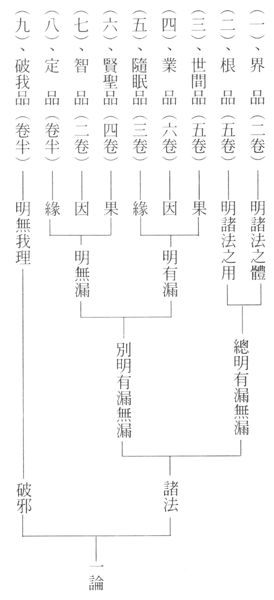
\includegraphics[scale=0.5]{释家/images/俱舍论科判.png}
\paragraph{《俱舍論》的品目記憶法,古來使用有一偈子}
\begin{quote}
「界二根五世間五,業六隨三賢聖四,\\
智二定二破我一,是名《俱舍》三十卷。」
\end{quote}
\subsubsection{《俱舍》的七十五法}
《俱舍論》將一切法分為有為法及無為法。凡依因緣造作而有時間的遷流,染淨的差別,即是一切世間的現象,均屬有為法;離有為法的性質,離一切作用的狀態,含有灰身滅智的涅槃義的,屬於無為法。
阿毘達磨多以五蘊、十二處、十八界的三科作為法的分類依準,《俱舍論》承此而復採用《品類足論》的色法、心法、心所有法、心不相應行法、無為法的五位,作為法的類別。
\footnote{七十五法的確定,是出於後來普光的《俱舍論記》,因為在《俱舍論》中,尚未將心所有法中的不定法之惡作、睡眠、尋、伺等做數字的確定。}
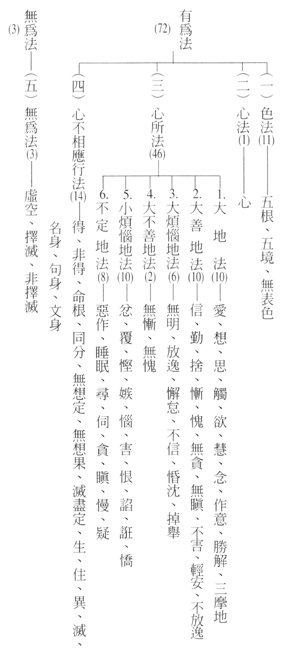
\includegraphics[scale=0.5]{释家/images/俱舍75法.png}
\subsubsection{《俱舍論》的〈世間品〉、〈業品〉、〈隨眠品〉}
是分析迷界的果、因、緣。迷界又分為有情世間及器世間。地獄、餓鬼、傍生、人、天,此五等為有情世間,乃為空間中的安立層次;有情的生死流轉,又分為生有、本有、死有、中有的四種狀態,依十二緣起而有三世兩重因果,乃是時間上的安立次第。欲界、色界、無色界,此三界為器世間在空間中的安立層次;又以成、住、壞、空的四劫,支配器世間的生滅循環,乃是器世間在時間上的安立次第。但是,若不出世間,世間法的安立,不論有情世間或器世間,總是迴還不已、無始無終、因果相續、因緣生滅。
眾生之不脫生死,是由造業而得的果報,本論的〈業品〉,即在對於業說的剖析。業分思業及思已業,意業為思業,身、語二業為思已業。又將身、語二業各各分為表業及無表業。
眾生之造業,是由於惑的驅使,本論的〈隨眠品〉,即為疏導惑的問題。隨眠是由業的活動而引生的苦果,它有煩惱的意味。煩惱分有根本的(六種或十種)及枝末的(十九種)。惑又分作迷理的見惑及迷事的修惑,見惑迷於四諦之理,配合三界則為八十八使;修惑即是根本煩惱中的貪、瞋、癡、慢的四種,三界共有十種,欲界四種,上二界除貪之外,各有三種。又有所謂百八煩惱,即是見惑的八十八使,加十種修惑及十纏而成。
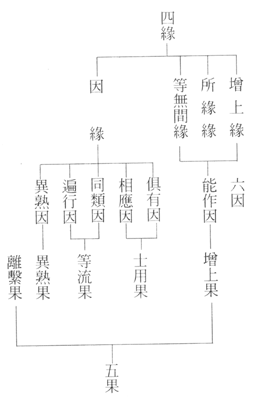
\includegraphics[scale=0.5]{释家/images/俱舍因缘论.png}
\subsubsection{《俱舍論》的〈賢聖品〉、〈智品〉、〈定品〉}
即是說明悟界的果、因、緣。智有決斷義,分為有漏智及無漏智。生得慧、聞慧、思慧、修慧的四種,稱為有漏智;法智、類智的二種,稱為無漏智。智的功能在斷見惑。至於定,分為生得定及修得定,此兩種定,
各有四色界定(四禪)及四無色界定,每一定又分有近分定及根本定。由智及定的功用,可漸次證入賢聖的果位,斷惑證真的階位過程極為繁複。
\footnote{無佛之世,有能自觀十二因緣而獨悟的聖者,稱為獨覺,梵名辟支迦佛(Pratyekabuddha)。釋尊的前生及至今生之尚未成佛以前,稱為菩薩,菩薩先修六度萬行,經三大阿僧祇劫,再經百劫植相好之業,最後證等正覺(成佛)。}
\begin{itemize}
  \item
    賢位七階,分作兩類
    \begin{enumerate}
      \item 三賢─五停心、別相念住、總相念住
      \item 四善根─煖善根、頂善根、忍善根(忍善根又可細分為下、中、上的三品)、世第一法。
    \end{enumerate}
  \item
    聖位兩類,分作三道八輩
    \begin{enumerate}
      \item 有學位分為見道的預流向,修道的預流果、一來向、一來果、不還向、不還果、阿羅漢向
      \item 無學位是無學道,即是阿羅漢果。這是有佛之世的聲聞果位。
    \end{enumerate}
\end{itemize}


\subsection{艺术}
原始佛教重修持、重解脫,未暇及於藝術;
由佛陀的悲智之中,流露出來的因緣觀,在在促使我們覺察我們所生存的空間和時間,乃由五蘊假合的身心而暫時存在,畢竟終歸於消滅,所以不要被外在的物質,色與聲所迷惑。


\subsubsection{佛像}
佛教,原來唯重人格精神的內在建設,不重形式的崇拜,所以原始的佛教,沒有任何祭祀的儀式,故也用不著偶像的崇拜。
\footnote{在早期的南印方面,仿照夜叉像而造佛像,所以頂上沒有肉髻相,多以獅子為座;在此後的北印方面,則仿照希臘神像而造佛像,頂有肉髻,以蓮花為座,有鬚有髮,此在西元前後四百年間,即形成了有名的犍陀羅的雕刻藝術。}

\subsubsection{文学作品}
《般若經》為否定的表現法,《法華經》、《維摩經》、《華嚴經》,採用象徵的表現法,《大無量壽經》則為感覺的表現法,密教的明咒乃是聲音的表現法。
佛傳如馬鳴的《佛所行讚》,乃是以優美的宮廷詩的格調寫成。《本生譚》則用民間故事的方式而寓佛教的意趣。

\subsection{大乘菩萨道}
\paragraph{有些大乘經典則並非出於佛說}
是由在家弟子的宣說而得到佛的印可,例如《維摩經》、《勝鬘經》便是
\footnote{佛經中也明白地顯示,佛法除了佛說的,尚有弟子說、仙人說、化人說、諸天說的。}
\footnote{因為小乘既由原始佛教而開出,也是大乘佛教的源頭,未必全是自私自了的小乘;大乘既有原始教理的根據,縱非皆出於佛說,何至於即成為魔說!}
。
\paragraph{般若思想為大乘的先河}
初期大乘聖典的漸次結集而公布於世,乃是一代又一代的具有進步思想的無名學者,他們在默默中為了發揚佛的本懷而工作。直到龍樹菩薩出世,集數百年無名大乘學者的工作成果於一身,予以蒐集整理著述發揚,才確立了大乘佛教的地位。
《般若經》通於大小三乘,也是大乘佛教之母。般若部所含經典極多,大至六百卷的《大般若經》,小至一張紙的《般若心經》。
般若的思想是一個「空」字,般若可譯為智,空即是智的客觀面,智是空的主觀面。有智必可證入空性,證入空性的必是智。所以智慧與空,畢竟是同一物的兩種名稱。
但是,般若的空,絕不等於虛無的世界觀及人生觀,而是基於緣生性空無所得的正觀,不受我執或我欲的困囚,以達到一種無礙自由的心境及其活動。

\subsubsection{净土思想}
彌陀淨土之確有其事,與西方極樂之究在何方,應是兩個問題。「生則定生,去則不去」,這是對西方之在何方的最好解答。

\subsubsection{入法界品}
文殊代表佛的智慧,普賢代表佛的行願,善財代表修證的人。由信而解,由解而行,由行而證;〈入法界品〉完成了學佛的四大階程。
華嚴的唯心,卻與西洋哲學的唯心,有所不同。因華嚴是基於緣起觀的立場,以清淨心為緣起的著眼,故也與般若的妄心緣起的立場不同。其他哲學的唯心論,則未嘗有緣起的觀念。緣起觀本為佛陀於菩提樹下所證悟的結果,由無明、行,而至老死,這可以稱為基於妄心而產生的「有」;若用真智觀照,此「有」是幻有,是空,般若的妄心緣起觀,即基於此一理論。可是經過「空」以後的緣起,從妙有的立場看,這個緣起,便是淨心緣起了。
\footnote{《華嚴經》即以為一即是一切,一切即是一;衝破時間及空間的藩籬,在一微塵中即含全法界,在一剎那間即含無窮遠;所謂芥子納須彌,須彌納芥子;所謂長劫入短劫,短劫入長劫}

\subsubsection{《維摩經》的立場}
繼《華嚴經》的思想,以全法界即是法身的顯現,而把佛法投向實際的人生,正好與小乘的逃脫人生的企圖相反。基於這個理由,便主張不捨道法而行凡夫之行,不斷煩惱而入於涅槃之境,能住於直心、深心、菩提心者,便是道場的禪定;真正的佛道,應從煩惱中、業中,發現佛種之所在。即煩惱而見菩提,不離生死而住涅槃。

\subsubsection{《妙法蓮華經》}
《華嚴經》及《維摩經》,站在大乘的立場,排斥二乘(聲聞、緣覺),《法華經》則起而做調停,欲使一切眾生向於佛乘,而仍不悖於大乘的使命,這就使三乘歸入一乘,表現了佛陀化世的本懷。不唯菩薩可成佛,聲聞弟子比丘、比丘尼,乃至畜道的龍女,也能成佛。三乘開會,力說悉皆成佛,這是本經被認作諸經之王的理由。

\subsubsection{淨土經典}
由來的聖典,都以現世的問題為中心,未嘗論及死後的救濟方法及其歸向;或以現世為出發點,而對未來永恆的彼岸,開始為佛陀或菩薩的淨土而經營,也未明白地指示死後去從的問題。
\begin{itemize}
  \item 彌勒(Maitreya 慈氏)的兜率淨土
  \item 阿閦(Aksobhya 不動)佛的東方淨土妙喜國
  \item 阿彌陀(Amitāyus, Amitābha 無量壽、無量光)佛的西方淨土極樂國\footnote{可以帶業往生,凡夫也能生彼國土,一切眾生凡能志信十念者即可往生。}
\end{itemize}

\subsubsection{中观学}
《中論》闡發緣起性空的深義,揭示生死解脫的根本,為三乘共由之門;《大智度論》採中道立場以顯不共般若;《十住毘婆沙論》以深遠之見而暢發菩薩之大行。
「月稱以先,雖有佛護、清辨諸家,性空猶和合無諍,彼此亦不自覺其有異。月稱獨契佛護,直標『此宗不共』之談,乃有『應成』、『自續』之諍」

\subsubsection{三期}
\begin{enumerate}
  \item 龙树之前
  \item 龙树到无著
    《如來藏經》\footnote{以勝鬘夫人為人物的中心,以闡說十大受、三大願為始,而來處理攝受正法、三乘方便、一乘真實,以及如來藏等的問題。}、
    《不增不減經》、《大法鼓經》、《勝鬘經》、《無上依經》、
    《大乘涅槃經》\footnote{大乘的《涅槃經》,乃由《長阿含經》的《遊行經》發展而來。對大乘而言,《遊行經》是小乘《涅槃經》;《遊行經》是以釋尊晚年的言行為主要的記錄,大乘《涅槃經》則不以事實的記述為中心,而以發揮其一定的教理為目的。}、
    《解深密經》、
    《入楞伽經》
    \footnote{主要觀念是在說明五法、三自性、八識、二無我。}
    \footnote{本經對於八個識均立有真相、業相、轉相之三相,其中真的本體,則是第八識的真相。前七識與第八識的業相、轉相,可由修行之力,特別是用人、法二空之觀法而消滅。消滅了這業相、轉相的當體,便是識海波浪的停止;它可叫作如來藏、真如、涅槃、法身、空、無垢識,乃是不生不滅、清淨無垢的當體。因此,本經是調和了如來藏思想與阿賴耶識思想,承認第八阿賴耶識含有淨與不淨兩方面的內容;從不淨方面,生起分別妄幻的現象界;從淨的方面又確立了法身、涅槃、真如的平等實體界。}
  \item 密教盛行
\end{enumerate}
當龍樹組織了大乘佛教,他的特色是破小乘而發揮大乘的優越性;到了無著,就把在教理方面開展到龍樹之上,同時也以小乘有部的繁瑣教理做基礎,而確立大乘佛教,乃是把小乘統合於大乘之內了。
\paragraph{為何稱唯識大乘為「瑜伽」?}這也與唯識學的環境及時代有關。凡是巧修止觀而有契入的,名為瑜伽師,為瑜伽師所依住的,名為瑜伽師地;可知,瑜伽師就是禪師,禪師多有內證的境界,故有從禪出教的事實,即是本於內證經驗而立說。小乘說一切有部的學者特深於禪,初來中國傳禪數之學的,也以西北印系的學者為主。

\subsubsection{唯识学}
唯識學發源於彌勒的《瑜伽師地論》,到了無著的《攝大乘論》而大成。此論是無著晚年的作品,有獨特的組織。此論是《大乘阿毘達磨經》之〈攝大乘品〉的釋論,乃是無著思想的代表作。內容共分十章,說明十種殊勝,並述有大乘佛教真是佛說的意趣。十種殊勝相可分為境、行、果的三類。一及二是境殊勝,三至八是行殊勝,九及十是果殊勝。
陳那對於因明的成就,更在唯識學之上,他的《集量論》(藏譯)及《因明正理門論》,改革了印度的舊因明而集印度論理學的大成。\footnote{尤其是《集量論》,不但在佛教有無上的價值,即在印度哲學史上也有極高的地位。}

\subsection{小乘 vs 大乘}
\paragraph{佛的時代,並無大小乘之分,只是一味的佛法} 由於弟子們的根器不同,對於佛法理解,才有不同的程度。從對象而言,佛陀對出家弟子所說的法,是著重於離世出世的,對在家弟子所說的法,是側重於和世樂群的,而其目標則同為解脫的涅槃境。因為佛陀的常隨弟子多是出家人,佛滅後初次結集(編集)佛經的,也全是出家人,故從原始聖典中,雖可得到大乘思想的消息,原則上毋寧是偏重於小乘的。
\paragraph{所謂小乘佛教,並非出現於佛世} 而是在佛陀入滅之後,出家僧團由於地域分布的不同影響,對佛的教法,產生了各各不同的異解,分張出許多的部派,小乘佛教,便是部派佛教。最先分為老比丘派的上座部與青年比丘派的大眾部,後來又從上座及大眾兩派之下,各自分出了許多部派,據《異部宗輪論》的介紹,共有二十個部派
\paragraph{在此許多部派的小乘佛教之中}以南印度的大眾部各派及流傳在西北印度的上座部下的一切有部,思想較為進步,故當著重於在家生活之教化的佛法再度復興之後,便是大乘佛教。南印的大眾部,即由小乘而漸漸地融入大乘。西北印的一切有部,也由小乘僧團之中,產生了許多大乘的宗師。
\paragraph{大乘佛教既然側重於和世樂群}大乘的精神,便是自度度人的菩薩行,菩薩行與世俗法,在表現上並無差別,只是在存心上有所不同。菩薩行是入俗而化俗,世俗法則是流俗而同於俗。所以,大乘的菩薩道,乃是外現世俗行,而內修解脫道的偉大法門。
\paragraph{在《阿含》聖典中,菩薩僅兩位}一是未成佛前的釋尊,一是當來在此世界成佛的彌勒;羅漢與佛的解脫雖同一味,羅漢終究不及佛的偉大,佛是由菩薩而成,菩薩也僅是指的未成佛前的釋尊;立有七佛,這是從古到今的多佛相次在人間成佛
\paragraph{大乘經教的特色}
小乘多用記事記實的文體,很少演繹鋪張。大乘經則多用通俗的演義、故事、譬喻、偈頌的文藝筆觸。
由大眾部到大乘教的許多論書,多有採取經的名稱而託為佛說,論書的性質與經書不同,是值得注意的。部派的小乘經典,在結尾時僅說明聞法者的歡喜奉行便止。大乘經典為使其廣為流佈起見,經末往往有「囑累」菩薩、天神、王臣等的護持,並且強調受持、讀誦、解說、書寫等的功德。
小乘教以羅漢的解脫為目標,大乘教則以菩薩道的圓滿─成佛為目標。所以,菩薩之道,深廣無倫,其主要內容為:菩薩,發菩提心,行六波羅蜜多,歷十地而成佛。
\footnote{《大智度論》的三句話可以總括大乘教義:1.一切智智相應作意─一切智智即是無上菩提;2.大悲為上首─發大悲心以普濟眾生之苦;3.無所得為方便行─體證緣生空無我之義,忘我而為眾生服役,嚴淨國土。}
\footnote{《大日如來經》,也有三句話攝大乘教義:1.菩提心為因,2.大悲為根本,3.方便為究竟。}

\subsection{那爛陀寺}
鳩摩利婆多的偉大著作是《吠陀真義評論》,婆羅門教的哲學因此大成,佛教的特色便因此消失,他雲遊全印,辯才無礙,弘揚其學說,攻破佛教。他是北印人,據說當他的南印派隆盛之時,佛弟子中竟無一人能夠勝過他們的議論;那爛陀寺的講學方式,一向公開,至此,因為無力降伏外道,只好改在內室講授。
\footnote{人能弘道,非道弘人,人才的優劣,與法運的隆污,關係實在太大了。}

\subsection{密教}
密教是頓悟法,也是易行道,它兼有求生西方淨土及印度教之與梵天合一的雙重優點。在歷程上是速成法,在目的上是究竟法。此一思想的形成,是在《大日經》的結集,大概是在西元第七世紀左右,由《大日經》而完成純密的理論,唱即身成佛。稍後出現《金剛頂經》而導發了後期的金剛乘,也就是左道密教。《大日經》的主要思想是「即事而真」,原則上是來自《華嚴經》的「事事無礙」,又參考梵我一致的印度教思想而進一步地唱出即身成佛之教。但《大日經》是密教理論的建設者,由《金剛頂經》開出的,即將此一理論付諸於實際的生活。一切都成為「即事而真」、「事事無礙」的結果,淫、怒、癡的現象,以為即是究竟的涅槃道。這在密教的理論上可以通,在究竟的佛位上也正確,在現實的凡夫境界,卻未必真的能夠「即事而真」。左道密教之濫,原因即在於凡聖混淆而倒果為因!
\subsubsection{法统}
密教最重視法統的師承,傳受密法,必須金剛上師(祕密阿闍梨)的灌頂,修持密法的儀軌,必須請金剛上師的加持,因為金剛上師是由師師相承而來的大日如來的代表,也必是修法有了成就的瑜伽行者。因為密教是心法,不同顯教可藉語文而領受,密教必須師弟祕密授受。
\subsubsection{瑜伽法}
瑜伽行者多有內證經驗,身心異於常人,所見也多屬實。唯其所驗,是否徹於佛的本懷,則有考察之餘地。因其重於心境的發現,境界固然屬實,若謂瑜伽行者的內證經驗,即是佛的境界而稱即身成佛,恐怕要落於增上慢了。這在佛世的小乘行者,由於修瑜伽法而自稱已證四果的,其實尚未離欲,佛陀不斥他們妄語,而稱之為增上慢人。
